
%%
%% INSTRUCOES
%%
%% Imagem Docker para compilar o documento:
%%
%% docker pull texlive/texlive
%%
%% Levantar o container:
%%
%% docker run -it --rm -v "${PWD}:/doc" -w /doc texlive/texlive bash
%%
%% Compilar o documento para PDF:
%%
%% pdflatex relatorio
%% bibtex relatorio
%% pdflatex relatorio
%% pdflatex relatorio
%%

\documentclass[a4paper, 12pt]{article}
%\documentclass[a4paper, 12pt]{report}

%%
%% PACOTES
%%
\usepackage[utf8]{inputenc}
\usepackage[T1]{fontenc}
\usepackage[utf8]{inputenc}
\usepackage[portuguese]{babel}
\usepackage{pdfpages} % incluir ficheiros PDF - para a capa
\usepackage{indentfirst} % identar a primeira linha
\usepackage[nottoc,numbib]{tocbibind} % referencias aparecerem no indice
\usepackage{url}

\usepackage{geometry}
\geometry{margin=2.5cm} % diminuir a margem

%%
%% METADADOS
%%

\title{Relatorio }
\author{Grupo}
\date{\today}

%%
%% INICIO DO DOCUMENTO
%%

\begin{document}

%% CAPA


\includepdf{capa/capa.pdf}

%% RESUMO


\begin{abstract}
O presente trabalho tem como objetivo analisar vulnerabilidades de segurança em aplicações desenvolvidas com a plataforma Base44, uma solução no-code baseada em inteligência artificial. A investigação centra-se no código do lado do cliente (frontend), procurando avaliar os riscos que podem existir mesmo sem acesso ao backend da aplicação.

A análise será conduzida segundo uma abordagem de testes de penetração do tipo caixa-cinzenta, adequada a contextos onde o acesso à infraestrutura é limitado. O estudo incidirá sobre falhas detetáveis através do navegador, como o armazenamento inseguro de dados, a manipulação inadequada do DOM e a exposição de recursos sensíveis. 

Com este projeto, pretende-se contribuir para uma maior consciência dos riscos inerentes ao desenvolvimento em plataformas no-code, sublinhando a importância da segurança mesmo em ambientes onde o controlo técnico do programador é reduzido.



\textbf{Keywords}: Segurança Web, Base44, Frontend, Cross-Site Scripting (XSS), LocalStorage, Service Worker.
\end{abstract}

%% INDICES

\tableofcontents

%\listoftables

\listoffigures

% CAPITULOS

\section{Introdução}

\subsection{Enquadramento e Propósito do Estudo}

O uso crescente de plataformas \textit{no-code}, como a Base44, veio simplificar o desenvolvimento de aplicações web, mas também trouxe novos desafios em termos de segurança. Estas soluções permitem que utilizadores construam aplicações funcionais sem qualquer contacto com o servidor ou com o código do \textit{backend}, o que reduz significativamente as possibilidades de análise e reforço da segurança.

Este estudo tem como objetivo analisar e avaliar vulnerabilidades existentes ao nível do \textit{frontend} de uma aplicação desenvolvida na Base44. Procura-se demonstrar que, mesmo com acesso apenas ao código do lado do cliente (\textit{HTML}, \textit{CSS} e \textit{JavaScript}), é possível identificar riscos que podem comprometer a integridade, a confidencialidade e a disponibilidade da aplicação.

O trabalho assume um carácter exploratório e prático, focando-se na reprodução de falhas reais e na implementação de soluções corretivas. O principal objetivo é contribuir para a consciencialização e para o reforço da segurança em ambientes \textit{no-code}, onde o controlo técnico por parte dos programadores é limitado, mas onde os riscos continuam a ser relevantes.

\subsection{Estrutura do Trabalho}

Após esta introdução, o relatório está organizado de forma lógica e progressiva, acompanhando o desenvolvimento do projeto desde os seus fundamentos teóricos até à análise prática dos resultados.

A secção seguinte apresenta uma visão geral das principais abordagens de teste de segurança web, com a explicação dos modelos de \textit{pentesting} utilizados na área: \textit{caixa-preta}, \textit{caixa-branca} e \textit{caixa-cinzenta}. Nesta parte, é também justificada a escolha da abordagem de \textit{caixa-cinzenta}, por se adequar ao contexto específico da aplicação analisada.

De seguida, serão detalhadas as ferramentas utilizadas no processo de análise, bem como a justificação técnica para a sua seleção.

Posteriormente, são apresentadas as vulnerabilidades identificadas na aplicação, cada uma acompanhada de uma explicação teórica, exemplos práticos e respetivas implicações de segurança.

Numa fase final, o relatório aborda vulnerabilidades previstas que não chegaram a ser confirmadas durante os testes e termina com uma reflexão crítica sobre as limitações da plataforma Base44, relacionando os resultados obtidos com os desafios mais amplos da segurança em ambientes \textit{no-code} baseados em inteligência artificial.


\section{Princípios de Avaliação da Segurança Web}

\subsection{Tipos de Testes de Penetração}

A avaliação da segurança em aplicações web recorre, frequentemente, a testes de penetração (\textit{pentesting}). Estes testes consistem na simulação controlada de ataques informáticos, com o objetivo de identificar vulnerabilidades que possam ser exploradas por atacantes. É uma prática fundamental em cibersegurança, pois permite analisar a capacidade de resistência de uma aplicação perante ameaças reais, sem comprometer o seu funcionamento.

Consoante o grau de acesso à aplicação, os testes de penetração podem ser classificados em três modelos principais \cite{ref53}:

\begin{flushleft}
\textbullet\ \textbf{Testes de Caixa-Preta (\textit{Black-box}):} Aqui o avaliador não tem qualquer informação interna sobre a aplicação, aproximando-se da perspetiva de um atacante externo. A análise é feita exclusivamente através da interação com a aplicação em execução, sem qualquer acesso ao código-fonte ou à documentação da arquitetura.

\vspace{0.4cm}

\textbullet\ \textbf{Testes de Caixa-Branca (\textit{White-box}):} Neste caso, o avaliador tem acesso total a todos os elementos do sistema, incluindo o código-fonte, bases de dados e configurações dos servidores. Permite uma análise exaustiva e é especialmente útil na deteção de falhas lógicas ou estruturais.

\vspace{0.4cm}

\textbullet\ \textbf{Testes de Caixa-Cinzenta (\textit{Grey-box}):} Este modelo híbrido trata-se de uma abordagem intermédia, em que o avaliador tem acesso parcial ao sistema. Por exemplo, poderá ter acesso ao código do \textit{frontend} ou a credenciais de utilizadores com permissões limitadas. A abordagem caixa-cinzenta representa um equilíbrio entre o realismo da caixa-preta e a profundidade da caixa-branca, sendo frequentemente considerada a mais eficiente em termos de custo-benefício em diversos cenários de teste.
\end{flushleft}

Estas abordagens são amplamente reconhecidas nas boas práticas de engenharia de software e de testes de segurança \cite{ref37}.

\subsection{Justificação da Abordagem Adotada: Caixa-Cinzenta (\textit{Grey-box})}

No âmbito deste projeto, a abordagem de caixa-cinzenta foi considerada a mais adequada, tendo em conta as restrições impostas pela plataforma Base44. Sendo uma solução \textit{no-code}, baseada em inteligência artificial, o acesso ao \textit{backend} e à configuração do servidor está bloqueado. No entanto, todo o código do lado do cliente (\textit{HTML}, \textit{CSS} e \textit{JavaScript}) está disponível, o que permite realizar uma análise focada no \textit{frontend}.

A imagem seguinte ajuda a visualizar, de forma esquemática, a abordagem adotada neste projeto.

\begin{figure}
    \centering
    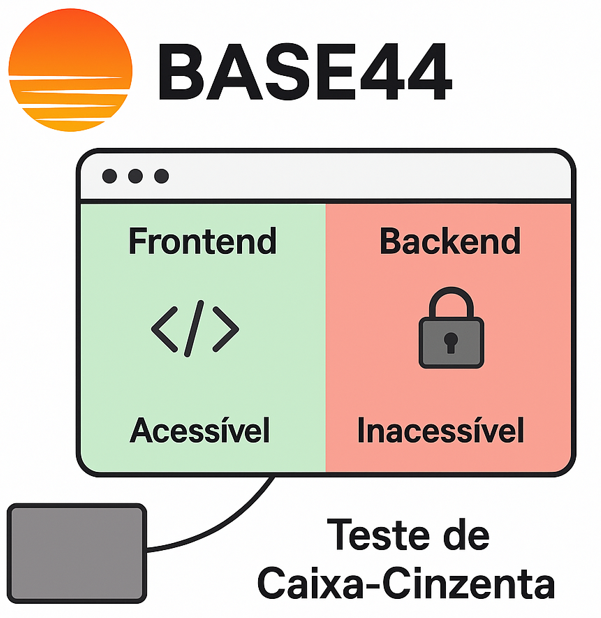
\includegraphics[width=0.4\linewidth]{imagens/diagrama.png}
    \caption{Representação esquemática da abordagem de caixa-cinzenta aplicada à Base44.}
    \label{fig:modelo_base44}
\end{figure}

Tal como representado na Figura~\ref{fig:modelo_base44}, apenas o \textit{frontend} da aplicação se encontra acessível para análise, enquanto o \textit{backend} permanece inacessível. Esta separação entre as duas camadas reflete as limitações impostas pela Base44 e ilustra bem a natureza da abordagem de caixa-cinzenta.

O diagrama reforça que, apesar do acesso restrito à infraestrutura do servidor, é possível aplicar técnicas de análise sobre os recursos disponíveis no lado do cliente. Esta abordagem equilibrada permite avaliar potenciais riscos de segurança de forma ética, segura e adequada ao contexto de plataformas \textit{no-code}.

A secção seguinte irá detalhar as ferramentas selecionadas, bem como a justificação técnica da sua utilização no âmbito do projeto.


\subsection{Métodos de Testes, Ferramentas Comuns e Abordagem Escolhida}

\subsubsection{Ferramentas automatizadas}

\paragraph{sqlmap}

é uma ferramenta automatizada
destinada à deteção e exploração de vulnerabilidades de injeção SQL em aplicações web.
Permite identificar parâmetros vulneráveis, avaliar técnicas de injeção
e, quando autorizado e possível, extrair dados a partir da base de dados alvo \cite{ref2}.
sqlmap é útil para demonstrar vetores de ataque e validar hipóteses de vulnerabilidade
em ambientes controlados; contudo, a sua utilização em sistemas de produção exige autorização explícita,
dado o elevado risco de impacto sobre a disponibilidade e confidencialidade dos dados \cite{ref3}.

\paragraph{nmap}
(Network Mapper) é uma ferramenta de mapeamento e descoberta de redes,
utilizada para identificar hosts ativos, portas abertas, serviços em execução e possíveis versões de software.
Fornece funcionalidades de reconhecimento essenciais nas fases iniciais de um teste de segurança \cite{ref1},
permitindo construir um inventário de superfície de ataque e orientar avaliações subsequentes.
nmap pode ser utilizado para ilustrar práticas de reconhecimento e perfilagem de rede,
mas deve ser usado com parcimónia e sempre dentro do âmbito autorizado,
pois varrimentos agressivos podem ser interpretados como atividade intrusiva.

\paragraph{nikto}

é um \textit{scanner} de servidores web orientado para a identificação de configurações incorretas,
ficheiros e \textit{endpoints} públicos potencialmente perigosos,
e componentes desatualizados com vulnerabilidades conhecidas \cite{ref2}.
Embora não tenha a sofisticação de \textit{scanners} comerciais,
é valioso para detetar rapidamente questões de configuração e itens de segurança negligenciados
que podem ser explorados em conjunção com outras falhas.
Para fins de investigação académica, nikto permite demonstrar vulnerabilidades de superfície web
e e problemas de \textit{hardening}, mantendo-se, tal como as outras ferramentas,
sujeito a restrições éticas e legais quando aplicado a sistemas
que não pertençam ao âmbito definido pelo estudo.

\subsubsection{Análise manual}
\paragraph{Revisão de código-fonte} — Leitura de ficheiros \textit{HTML}, \textit{JavaScript} e de configuração
para identificar segredos expostos \cite{ref12}, padrões inseguros ou lógica vulnerável no lado do cliente.
\paragraph{Ferramentas de programador do navegador} — Utilizadas para inspecionar o DOM,
pedidos de rede, \textit{cookies}, armazenamento local (\textit{localStorage}/\textit{sessionStorage})
e a execução de \textit{JavaScript}, permitindo observar o comportamento em tempo real
e potenciais falhas no \textit{frontend} \cite{ref1}.

\subsubsection{Testes estáticos vs. dinâmicos}
\paragraph{Testes estáticos} analisam o código e artefactos sem os executar
(por exemplo, revisão de \textit{JS}/\textit{HTML}, pesquisa de segredos, análise de mapas de origem \cite{ref20}).
São de baixo impacto e adequados quando apenas estão disponíveis recursos do lado do cliente.
\paragraph{Testes dinâmicos} envolvem interação direta com sistemas em execução
(por exemplo, injeção de \textit{payloads}, \textit{fuzzing} de \textit{endpoints}, exploração de lógica no servidor).
Embora possam identificar vulnerabilidades em tempo real,
implicam maior risco e requerem autorização explícita \cite{ref4}.

\subsection{Justificação da Abordagem Escolhida}
Tendo em conta que o presente estudo incide sobre aplicações exportadas da plataforma Base44 \cite{ref16},
o acesso disponível limita-se aos componentes do \textit{frontend}.
Por este motivo, a abordagem escolhida foca-se na análise estática de baixo impacto,
complementada com sondagens manuais seguras,
garantindo que todas as atividades são realizadas de forma ética e sem afetar
a integridade do ambiente de alojamento.

Será utilizada a combinação de ferramentas e técnicas seguintes:
as \textit{DevTools} do navegador para inspeção de \textit{localStorage},
\textit{service workers} \cite{ref8} e \textit{cache};
\textit{Burp Suite} ou \textit{OWASP ZAP} \cite{ref23} para varrimento controlado
de vulnerabilidades e verificação das evidências;
\textit{DOMPurify} em conjunto com a aplicação de cabeçalhos CSP \cite{ref25}
para mitigação de XSS;
e um \textit{nginx} auto-alojado para forçar \textit{TLS 1.3}
e configurar cabeçalhos de segurança \cite{ref19} no nível do servidor.

Ferramentas e técnicas que requerem interações com o \textit{backend},
como \textit{sqlmap} (injeção \textit{SQL}), \textit{nikto} (\textit{scanner web} dinâmico)
ou \textit{nmap} (varrimentos de rede), foram consideradas, mas não serão utilizadas,
pois excedem o âmbito do projeto e não são compatíveis com a política de ética e segurança definida.

Assim sendo, a abordagem selecionada permite avaliar de forma responsável e ética
a superfície de ataque do \textit{frontend} das aplicações Base44,
identificar vulnerabilidades relevantes e aplicar correções demonstráveis,
enquanto se minimiza o risco de impacto sobre o ambiente de alojamento
ou os dados dos utilizadores \cite{ref27}.
Esta escolha garante que os objetivos do projeto — "reproduzir, corrigir e documentar
vulnerabilidades de forma segura e eficaz” — podem ser atingidos
dentro do período de execução previsto.

\newpage

\section{Vulnerabilidades Detetadas no Projeto}
\label{sec:vulnerabilidades-detetadas}

\subsection{DOM-based XSS}
\label{subsec:dom-based-xss}

O Cross-site Scripting (XSS) é uma das vulnerabilidades mais comuns em aplicações web, estando consistentemente no Top 10 da OWASP. Esta vulnerabilidade permite que atacantes injetem código malicioso (geralmente JavaScript) em páginas web visualizadas por outros utilizadores, comprometendo a integridade da aplicação e a segurança dos dados.

O DOM-based XSS representa uma variante específica desta vulnerabilidade, em que o ataque ocorre inteiramente no lado do cliente, ou seja, no navegador do utilizador. Ao contrário das abordagens tradicionais de XSS (refletido ou armazenado), que exploram respostas do servidor, o DOM-based XSS resulta de manipulações inseguras feitas pelo próprio código JavaScript da aplicação \cite{ref39}.

Neste tipo de ataque, o JavaScript lê dados potencialmente maliciosos provenientes de fontes como parâmetros do URL (\texttt{location.search}), fragmentos do URL (\texttt{location.hash}), armazenamento local (\texttt{localStorage}, \texttt{sessionStorage}) e mensagens recebidas via \texttt{postMessage}.

Estes dados são então inseridos diretamente no DOM através de funções conhecidas como \textit{sinks} inseguros, como o \texttt{innerHTML}, \texttt{outerHTML}, \texttt{insertAdjacentHTML}, \texttt{document.write}, \texttt{eval}, \texttt{new Function} e APIs que interpretam HTML ou JavaScript \cite{ref40}.

Se esses dados não forem devidamente validados e tratados, o navegador pode interpretar e executar o conteúdo malicioso, resultando em execução de código não autorizado \cite{ref38}.

\subsubsection{Riscos e Impacto dos Ataques DOM-based XSS}
\label{subsubsec:riscos-impacto-dom-xss}

Os ataques DOM-based XSS representam uma ameaça significativa à segurança das aplicações web, especialmente quando estas manipulam dados sensíveis ou sessões de utilizadores. Estes ataques podem ser explorados para:

\begin{itemize}
    \item \textbf{Roubo de dados} em que código malicioso pode ser executado no contexto da aplicação, permitindo o acesso a cookies (caso não estejam protegidos com a flag \texttt{HttpOnly}), tokens armazenados no \texttt{localStorage} ou \texttt{sessionStorage}, e outros dados confidenciais.
    
    \item \textbf{Manipulação da interface} pois o atacante pode alterar elementos visuais da página, simulando interfaces legítimas para enganar o utilizador (phishing).
    
    \item \textbf{Execução de ações não autorizadas} porque é possível orquestrar ataques como CSRF ou SSRF, explorando a confiança do navegador na origem da aplicação.
\end{itemize}

Esta vulnerabilidade é particularmente difícil de detetar, pois não envolve comunicação com o servidor, fazendo com que o código malicioso seja processado e executado exclusivamente no cliente \cite{ref39}. Além disso, como o código gerado por plataformas no-code (como a Base44) é frequentemente compilado e abstraído, torna-se ainda mais desafiante identificar e corrigir estas falhas.

\subsubsection{Boas práticas de prevenção}
\label{subsubsec:boas-praticas-prevencao-dom-xss}

A mitigação eficaz de DOM-based XSS deve ser integrada desde a fase de arquitetura até ao ciclo de desenvolvimento. Algumas estratégias recomendadas incluem \cite{ref40}, \cite{ref41}:

\begin{itemize}
    \item \textbf{Uso de APIs seguras} em que são preferíveis métodos como \texttt{textContent}, \texttt{setAttribute} (com validação), \texttt{value} para campos de formulário, e \texttt{createElement} com \texttt{appendChild}, em vez de \texttt{innerHTML} ou \texttt{eval}.
    
    \item \textbf{Tratamento robusto de dados} utilizando bibliotecas confiáveis com listas de permissões (\textit{allowlists}) para limpar dados antes de os inserir no DOM. Evitar soluções caseiras baseadas em expressões regulares, que são frequentemente insuficientes.
    
    \item \textbf{Codificação por contexto} em que se aplica \textit{output encoding} adequado ao tipo de conteúdo quer seja HTML, atributos, URLs, CSS ou JavaScript de modo a evitar interpretações indevidas.
    
    \item \textbf{Eliminação de funções perigosas} para isto evita-se completamente o uso de \texttt{eval} e \texttt{new Function}. Caso sejam indispensáveis, devem ser isoladas em ambientes controlados.
    
    \item \textbf{Políticas de segurança no navegador} implementando cabeçalhos como CSP com \textit{nonce} ou \textit{hash}, que ajudam a bloquear scripts injetados. Complementar com \texttt{X-Content-Type-Options: nosniff}, \texttt{Referrer-Policy} e \texttt{Permissions-Policy} para reduzir a superfície de ataque.
    
    \item \textbf{Minimização da superfície de confiança} limitando o acesso a fontes como \texttt{location}, \texttt{document.referrer} e \texttt{localStorage}, e validar rigorosamente o formato dos dados recebidos.
\end{itemize}

\subsubsection{Metodologias de teste}
\label{subsubsec:metodologias-teste-dom-xss}

A identificação de vulnerabilidades DOM-based XSS requer uma combinação de técnicas manuais e automáticas como \cite{ref38}, \cite{ref42}:

\begin{enumerate}
    \item \textbf{Mapeamento de fontes e sinks} em que se identifica onde os dados entram na aplicação (ex.: \texttt{location.search}, \texttt{postMessage}, inputs do utilizador) e onde são inseridos no DOM (ex.: \texttt{innerHTML}, \texttt{eval}, \texttt{insertAdjacentHTML}).
    
    \item \textbf{Revisão estática do código} analisando o JavaScript compilado ou minificado, procurando padrões perigosos. Ferramentas como \textit{source maps} ou \textit{prettifiers} podem ajudar a tornar o código mais legível.
    
    \item \textbf{Instrumentação dinâmica} recorrendo ferramentas como o DOM Invader (Burp Suite) ou DevTools para observar o comportamento do código em tempo real e seguir o caminho dos dados até aos \textit{sinks}.
    
    \item \textbf{Testes manuais seguros} em que se injetam marcadores identificáveis (ex.: \texttt{INJECTION\_TEST\_123}) nos pontos de entrada e se verifica se aparecem no DOM sem codificação adequada.
    
    \item \textbf{Ferramentas automáticas} e neste âmbito existem scanners especializados em DOM-XSS, como proposto por Melicher et al. \cite{ref42}, linters com plugins de segurança (ex.: ESLint), e ferramentas de análise de dependências para verificar bibliotecas externas que manipulam HTML.
    
    \item \textbf{Avaliação de mitigadores} confirmando que as políticas de segurança estão ativas e são eficazes, e que os métodos seguros estão a ser utilizados corretamente.
\end{enumerate}

\subsection{Potential Open Redirects}
\label{subsec:potential-open-redirects}

Os redirecionamentos abertos (\textit{open redirects}) constituem uma vulnerabilidade lógica que ocorre quando uma aplicação permite que o utilizador seja redirecionado para um URL externo, com base num parâmetro do URL, sem validação adequada. Esta falha pode ser explorada por atacantes para conduzir utilizadores a sites maliciosos, disfarçando o destino real por trás de um domínio legítimo. Embora não envolva execução de código diretamente, o impacto pode ser significativo, sobretudo em contextos de phishing, onde a confiança do utilizador na aplicação é essencial.

Durante a análise da aplicação desenvolvida com a plataforma Base44, foram identificadas estruturas de código que utilizam variáveis como \texttt{redirect} e \texttt{URL} na lógica de navegação. Embora não tenha sido demonstrada uma exploração direta, a presença destas variáveis sugere que o sistema pode aceitar valores externos para redirecionamento, o que representa um vetor de ataque potencial. Esta preocupação é corroborada por Khodayari et al. \cite{ref43}, que demonstram como redirecionamentos abertos podem ser explorados de forma sofisticada, desafiando a perceção comum de que são inofensivos.

\subsubsection{Riscos e implicações}
\label{subsubsec:riscos-implicacoes-open-redirects}

Os \textit{open redirects} podem ser explorados em diversos cenários:

\begin{itemize}
    \item Em ataques de \textbf{phishing}, o atacante pode enviar um link aparentemente legítimo que redireciona para uma página falsa, capturando credenciais do utilizador \cite{ref44}.
    
    \item Em sistemas de segurança baseados em listas de permissões, os users podem ser enganados, confiando no domínio inicial sem verificar o destino final \cite{ref43}.
    
    \item Em fluxos de autenticação como OAuth ou SSO, redirecionamentos mal validados podem permitir a captura de tokens de sessão \cite{ref45}.
    
    \item Além disso, o domínio legítimo pode ser usado para disseminar links maliciosos, afetando a reputação da aplicação.
\end{itemize}

\subsubsection{Estratégias de mitigação}
\label{subsubsec:estrategias-mitigacao-open-redirects}

A mitigação desta vulnerabilidade passa por várias abordagens:

\begin{itemize}
    \item \textbf{Listas de destinos permitidos}: A abordagem mais eficaz consiste na utilização de \textit{allowlists}, validando se o destino pertence a um conjunto de domínios ou caminhos autorizados \cite{ref45}.
    
    \item \textbf{Uso de caminhos relativos}: É recomendável o uso de caminhos relativos, como \texttt{next=/dashboard}, e a validação com \texttt{startsWith('/')}.
    
    \item \textbf{Evitar redirecionamentos arbitrários}: Em fluxos sensíveis, como a autenticação ou recuperação de senha, deve-se evitar redirecionamentos arbitrários.
    
    \item \textbf{Tokenização}: Uma alternativa segura é a tokenização, onde o parâmetro recebido é um identificador que mapeia para um URL seguro armazenado no servidor \cite{ref43}.
    
    \item \textbf{Validação rigorosa}: Deve incluir a canonicalização do URL, bloqueando esquemas perigosos como \texttt{javascript:} ou \texttt{data:} \cite{ref45}.
    
    \item \textbf{Página intermediária}: Em casos onde o redirecionamento externo é necessário, é aconselhável apresentar uma página intermediária que informe o utilizador sobre o destino, promovendo a transparência e reduzindo o risco de \textit{Social Engineering} \cite{ref44}.
\end{itemize}

\subsubsection{Metodologia de Teste}
\label{subsubsec:metodologia-teste-open-redirects}

A deteção de \textit{open redirects} pode ser realizada através de:

\begin{itemize}
    \item \textbf{Revisão de código}: procurando por padrões como \texttt{location.href}, \texttt{window.location}, \texttt{res.redirect}, \texttt{window.open}, entre outros \cite{ref46}.
    
    \item \textbf{Testes manuais}: consistem em injetar parâmetros controlados e observar o comportamento da aplicação, verificando se o redirecionamento ocorre sem validação.
    
    \item \textbf{Testes de bypass}: incluem variações como \texttt{//malicioso.com}, URLs com \texttt{@}, codificações Unicode ou esquemas obsoletos \cite{ref47}.
    
    \item \textbf{Validação de fluxos OAuth/SSO}: é essencial confirmar se o parâmetro \texttt{redirect\_uri} é validado contra uma lista segura \cite{ref45}.
    
    \item \textbf{Ferramentas automáticas}: como Burp Suite, ZAP e linters estáticos podem auxiliar na identificação de padrões vulneráveis \cite{ref48}.
    
    \item \textbf{Precauções durante testes}: é fundamental evitar redirecionamentos para domínios maliciosos, utilizando marcadores inócuos e documentando os passos de reprodução \cite{ref49}.
\end{itemize}

\section{Vulnerabilidades Testadas mas Não Detetadas}

Durante a análise de segurança à aplicação alojada na plataforma Base44, foram também considerados outros vetores de ataque comuns em aplicações web modernas, com o objetivo de realizar uma avaliação mais abrangente e alinhada com as boas práticas internacionais de segurança \cite{ref1, ref2}.

Ainda que não tenham sido identificadas ocorrências dessas vulnerabilidades no projeto em análise, a sua inclusão demonstra uma abordagem metodológica informada e coerente com os princípios do OWASP e das normas NIST \cite{ref3, ref4}.

Segue-se o resumo das vulnerabilidades analisadas, precedido por uma breve descrição teórica de cada uma.

\subsection{CORS Mal Configurado (\textit{Cross-Origin Resource Sharing})}

\subsubsection{Enquadramento Teórico}

O \textit{Cross-Origin Resource Sharing} (CORS) é um mecanismo de segurança implementado nos navegadores modernos que controla como recursos (por exemplo, dados de APIs) podem ser solicitados entre diferentes origens (\textit{origins}) \cite{ref5}.

Sem CORS, o \textit{Same-Origin Policy} (SOP) impede que \textit{scripts} executados numa origem (e.g., \url{https://app.example.com}) acedam a recursos noutra (e.g., \url{https://api.example.org}).

Uma configuração incorreta de CORS pode permitir que um domínio malicioso obtenha dados sensíveis através de pedidos legítimos, violando a confidencialidade da aplicação. Exemplos comuns incluem:
\begin{itemize}

\item Cabeçalhos permissivos, como Access-Control-Allow-Origin: *;

\item Reflexão do valor de \textit{Origin} sem validação;

\item Permissão de cabeçalhos ou métodos inseguros.

\end{itemize}

\subsubsection{Análise Realizada}

Foi efetuado um teste manual utilizando o comando cURL com cabeçalhos personalizados de \textit{Origin}, de forma a verificar se o servidor aceitava requisições de domínios externos sem validação adequada.\\

\verb!curl -I -H "Origin: http://malicious.example.com" https://app.base44.io!\\

Durante os testes, não foram detetadas configurações permissivas, nem cabeçalhos vulneráveis. Conclui-se que a aplicação não apresenta fragilidades relacionadas com CORS nesta fase \cite{ref7}.

\subsection{Riscos Associados a \textit{Service Workers e Cache Storage}}

\subsubsection{Enquadramento Teórico}

Os \textit{Service Workers} são \textit{scripts} registados pelo navegador que atuam como \textit{proxies} entre a aplicação e a rede, permitindo funcionalidades como execução \textit{offline}, \textit{background synchronization} e \textit{push notifications} \cite{ref8}.

Embora úteis, podem introduzir riscos de segurança se mal configurados - nomeadamente:

\begin{itemize}

\item \textit{Cache poisoning}, quando conteúdo malicioso é armazenado e servido como legítimo;

\item \textit{Persistent malicious scripts}, que se mantêm mesmo após correções no servidor;

\item Manutenção indevida de dados sensíveis em \textit{Cache Storage}.

\end{itemize}

Uma aplicação que utilize \textit{Service Workers} deve assegurar controlos de integridade, âmbito restrito e atualização segura \cite{ref9}.

\subsubsection{Análise Realizada}

A análise ao código-fonte revelou ausência de qualquer registo ou implementação de \textit{Service Workers} e de uso explícito da \textit{Cache Storage API}, tornando este vetor não aplicável a este projeto em análise.

Consequentemente, os riscos associados a \textit{offline persistence} ou manipulação de \textit{cache} são inexistentes nesta fase.

\subsection{Vulnerabilidades em \textit{Scripts} de Terceiros}

\subsubsection{Enquadramento Teórico}

Bibliotecas e \textit{frameworks} de terceiros são componentes fundamentais no desenvolvimento web, mas também representam um dos principais meios de ataque modernos \cite{ref10}.

Ataques à cadeia de fornecimento (\textit{supply chain attacks}) podem ocorrer quando uma dependência legítima é comprometida, afetando todas as aplicações que a utilizam.

Outros riscos incluem:

\begin{itemize}

\item Inclusão de versões desatualizadas com vulnerabilidades conhecidas (CVE);

\item Hospedagem de \textit{scripts} em CDNs não confiáveis;

\item Modificação de dependências por terceiros não autorizados.

\end{itemize}

A OWASP recomenda o uso de ferramentas de verificação de dependências e auditorias regulares para reduzir esse risco \cite{ref11}.

\subsubsection{Análise Realizada}

Foi conduzida uma inspeção estática e dinâmica aos ficheiros JavaScript utilizados na aplicação, com foco nas dependências externas.

Verificou-se que apenas foram incluídas versões oficiais hospedadas em CDNs reputadas, como jsDelivr e Cloudflare.

Não foram encontradas bibliotecas desatualizadas ou modificadas, reduzindo significativamente o risco de exploração.

\subsection{Exposição de \textit{Tokens} ou API \textit{keys}}

\subsubsection{Enquadramento Teórico}

A exposição de segredos (como \textit{tokens}, API \textit{keys} ou credenciais) é uma das falhas mais comuns em aplicações web e representa uma ameaça direta à integridade e confidencialidade do sistema \cite{ref12}.

Quando segredos estão embutidos no código-fonte — especialmente no \textit{frontend} — tornam-se acessíveis a qualquer utilizador que inspecione o código, permitindo:

\begin{itemize}

\item Autenticação não autorizada em APIs;

\item Acesso a dados confidenciais;

\item Comprometimento de outros serviços integrados.

\end{itemize}

A OWASP recomenda a gestão centralizada de segredos, armazenamento seguro no servidor e rotação periódica de chaves \cite{ref13}.

\subsubsection{Análise Realizada}

Durante a análise estática do código-fonte (HTML, JavaScript e cabeçalhos HTTP), procuraram-se padrões típicos de exposição de segredos, incluindo termos como \textit{apiKey}, \textit{token}, \textit{Authorization}, e chaves codificadas em Base64.

Foram efetuadas pesquisas manuais e automatizadas, incluindo inspeção de ficheiros minificados.

Não foram identificados valores sensíveis embutidos no código, o que demonstra uma boa segregação de segredos e práticas seguras de gestão de credenciais \cite{ref14, ref15}.

\subsection{Conclusão}

Embora nenhuma destas vulnerabilidades tenha sido identificada na aplicação analisada, a sua verificação foi essencial para garantir uma abordagem responsável, abrangente e conforme as normas internacionais de segurança.

Os resultados reforçam que, mesmo em ambientes \textit{no-code} e com integração de IA, é possível seguir metodologias de análise de risco alinhadas com os princípios do OWASP Top 10 (2021) e do NIST Cybersecurity Framework (CSF) \cite{ref2, ref4}.


\section{Questões Conhecidas e Reportadas ao Nível da Plataforma (Base44)}

% BIBLIOGRAFIA

\bibliography{bibliografia/biblio}{}
\bibliographystyle{IEEEtran}

%%
%% FIM DO DOCUMENTO
%%
\end{document}
